\documentclass[border=10pt]{standalone}
\usepackage{tikz}
\usetikzlibrary{shapes, positioning, arrows.meta, calc}

\begin{document}
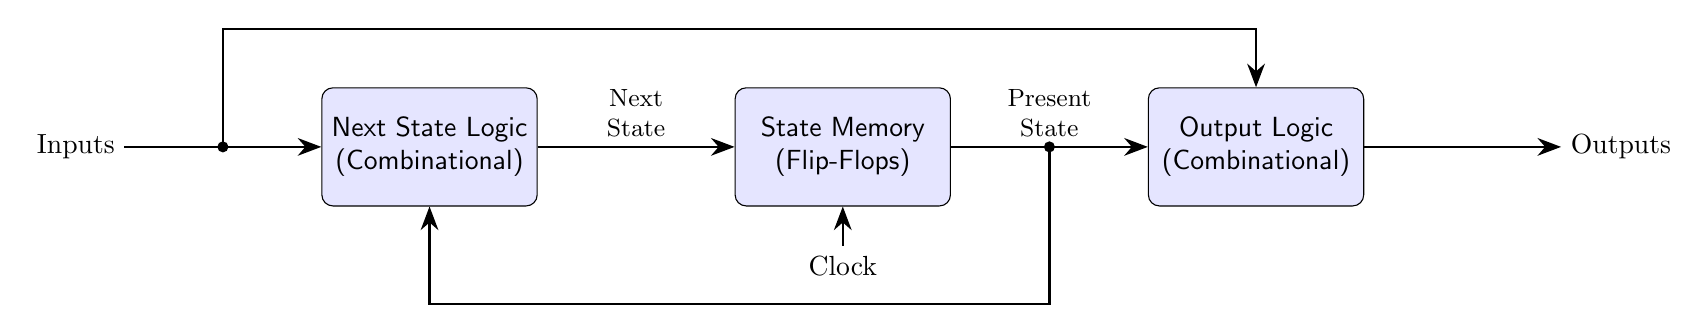
\begin{tikzpicture}[
    auto,
    block/.style={rectangle, draw, fill=blue!10, text width=2.5cm, text centered, rounded corners, minimum height=1.5cm, font=\sffamily},
    line/.style={draw, -{Stealth[length=3mm]}, thick},
    node distance=2.5cm
]

    % Nodes
    \node (input) {Inputs};
    \node [block, right=of input] (nextstate) {Next State Logic\\(Combinational)};
    \node [block, right=of nextstate] (memory) {State Memory\\(Flip-Flops)};
    \node [block, right=of memory] (outputlog) {Output Logic\\(Combinational)};
    \node [right=of outputlog] (output) {Outputs};

    % Main horizontal path
    \draw [line] (input) -- (nextstate);
    \draw [line] (nextstate) -- node[midway, align=center, font=\small] {Next\\State} (memory);
    \draw [line] (memory) -- coordinate(mid) node[midway, align=center, font=\small] {Present\\State} (outputlog);
    \draw [line] (outputlog) -- (output);
    
    % Feedback Loop
    \fill (mid) circle (2pt);
    \draw [line] (mid) -- ++(0,-2) -| (nextstate.south);
    
    % Input feed to Output Logic (General FSM includes Mealy)
    \draw [line] ($(input.east)!0.5!(nextstate.west)$) coordinate(split) -- ++(0, 1.5) -| (outputlog.north);
    \fill (split) circle (2pt);

    % Clock signal
    \draw [line] ($(memory.south) + (0, -0.5)$) node[below] {Clock} -- (memory.south);
    % Clock triangle
    %\draw ($(memory.south) + (-0.1, 0)$) -- ($(memory.south) + (0, 0.2)$) -- ($(memory.south) + (0.1, 0)$);

\end{tikzpicture}
\end{document}
